\documentclass[Journal,InsideFigs, DoubleSpace]{ascelike} %NewProceedings, Journal
%figs in the back \documentclass[Journal, BackFigs, DoubleSpace]{ascelike} %NewProceedings, Journal

%include package for inserting picture
\usepackage{graphicx}%insert image
\DeclareGraphicsExtensions{.pdf,.png,.jpg}
\graphicspath{{figures/}}%folder contains images

\usepackage{caption}%packages for inserting multiple pictures
\usepackage{subcaption}%packages for inserting multiple pictures

\usepackage{array}%for table with fixed width
\newcolumntype{L}[1]{>{\raggedright\let\newline\\\arraybackslash\hspace{0pt}}m{#1}}
\newcolumntype{C}[1]{>{\centering\let\newline\\\arraybackslash\hspace{0pt}}m{#1}}
\newcolumntype{R}[1]{>{\raggedleft\let\newline\\\arraybackslash\hspace{0pt}}m{#1}}

\usepackage{amsmath} %math package

\usepackage{algorithm} %algorithm package
\usepackage[noend]{algpseudocode} % pseudo code package

\usepackage[utf8]{inputenc}%french accents
\usepackage[T1]{fontenc} %for accented characters

\usepackage{booktabs}%allowing drawing hline in table crossing only some columns

\usepackage{enumitem}


\begin{document}

\title{NLP-based approach to structuring heterogeneous terms \\for unambiguous exchange of highway data}

% automated generation of highway lexicon classifying lexical relationships between heterogeneous highway technical terms lexicon generation , inconsistency  \\in highway projects}

%
\author{
Tuyen Le
\thanks{
Ph.D. Candidate, Department of Civil, Construction and Environmental Engineering, Iowa State University. Ames, IA 50011, United States. E-mail: ttle@iastate.edu.},
\and
H. David Jeong
\thanks{Associate Professor, Department of Civil, Construction and Environmental Engineering, Iowa State University. Ames, IA 50011, United States. E-mail: djeong@iastate.edu.}
 }

\maketitle
%
%\begin{center}
%(To be submitted to the Journal of Computing in Civil Engineering) 
%\end{center}

\begin{abstract} %150-175 words (as required by ASCE)
%background:
The inconsistency of data terminology due to the fragmented nature of the civil infrastructure industry has imposed big challenges on integrating digital data from distinct sources to support decision making in asset management. The issue of data ambiguity may lead to a lack of common understanding to the same data between the sender and receiver. While the heterogeneity of data formats has been well addressed thanks to the availability of various international neutral data standards such as LandXML and TransXML;  the heterogeneity of terms where various terms used from the same concept still has been neglected by the domain researchers. 
%research objective
This paper presents a novel methodology to construct an automatically-generated lexicon, namely InfraLex, that formally organizes civil infrastructure technical terms in a lexical hierarchy manner. The lexicon severs as a digital dictionary of domain terms which would enable data integration systems to understand the meaning of a data representation, and helps avoid the mismatch of data.
%research methods
Natural Language Processing (NLP) techniques and the C-value method are used to detect technical terms from a highway text corpus collected from roadway design guidelines across the State Departments of Transportation. A model for measuring term similarity is trained using the Skip-gram model which uses the corpus as the training dataset. This semantic model is then utilized by a term classification algorithm that organizes related terms into separate groups according to their semantic relations.
%result
The developed lexicon was evaluated by conducting an experiment comparing the automatically-identified synonyms with a human-constructed synonym set. The result shows that the proposed model achieved a precision of over 80 percent.
  
\end{abstract}

\KeyWords{Civil infrastructure project, Lexicon, Data sharing, Semantic Interoperability, NLP, Vector Space Model}
%
%\newpage


%********************************************************
%good terms and phrases:

%adj: nonhierarchical, superior, well-defined; foreseeable; rigid, flexible, empirical, disparate, isolated, labrious and resouce-intensive, proprietary, integrated, shared, inefficent, time-consuming, laborious, prone error, consistent, easy-to-use, intuitive solutions, extensive, transformative impact, labour extensive, 

%sentence structure:  this is evidenced by the accelerating emergence of ...; 

%noun: challenges, barrier, hinders, obstacles, impediment; that approximate concepts; extraction=deduction=acquisition; broad spectrum; overtake these technical and economic challenges; bottleneck; data crreation and utilization; in the midst of planning; interpretation; multitude of data,  data repository, a structured system of terms, data representation, initiatives, bottleneck, insight and value from massive amounts of data, technology and skillset, data scale, magnitude,  a plethora of, data sharing pardigm, inconsistency, discrepancy, the origin of, vicinity=neigborhood, very little of st, 

%verb: emcombass; tackle, foster, amplified; simplified; detect; aggregate; encompass, manifest,envision,  is divided into two, is shared among,  derive, extract, eunsure data to be understood, 

%adv: namely, undoubtedly, oftentimes, cohesively, extensively,

%linking: thereby, only those concepts that, whereby, 

%sentence template: tailored with respect to their context; includes three phases, namely AA, BB and CC; at such places as parks, fairgounds or town spuares; case-specific developments; area of interests; incrementally built; inexpensive and easy-to-use testing device; time and cost-efficient way; research community; one of..since then is the; RDF structure..to make assertion about a resource; syntax-centered NLP;  such as A, B, etc.; ..is in it's reliance upon the presence..which is..; with the objectives of disambiguation; has triggered a mounting awareness; to be the main impediment to the progess; ..start point for deducing other truth; lastly; there is a large body of research on; see e.g. [2], [14] and [32]; the former, the latter; rigorously formalized; backbone strucutre of st; was opted to; Sections 4.5 and 4.6; (e.g., Neo4J, OrientDB, Titan); forthcoming year; well-designed process; is subject to do st; in turn means that; discussion by academics and professionals; some insights on planning, management, and control; strategic framework; in-depth project performance; in lieu of; 

%term': empirical work; linguistic unit/term; 

%axiomatic richness, formality of representation,  

%the following expression denotes, is presented/defined as follows, this/below example shows, the snippet below presents, the following is the short description of the rule, an OWL ontology describing an ifcwindow class, these concepts and relationships can be encoded in the following RDF/XML fragment, is written in Turtle syntax/format:
%The tool is meant to assess, 
%********************************************************

\section{Introduction}%900 words
%Topic introduction, territory: centrality--> general background information 
%the background of data extraction
The implementation of advanced computerized technologies such as 3D modeling and Geographic Information System (GIS) throughout the life cycle of a civil infrastructure project has allowed a large portion of project data to be available in digital format. The efficiency improvement in sharing these data between project participants and stages, will in turn, translate into increased productivity, efficiency in project delivery and accountability. However, a highway asset as a whole has not yet fully benefited from the potentials of digital datasets as an accessible, reusable and reliable information source for life-cycle decision making due to the interoperability issue. A study by the National Institute of Standard and Technology (NIST) reported an estimated inadequate interoperability cost in the U.S. capital facility industry at over \$15.8 billion per year \cite{Gallaher04}. This study also pointed out that two-third of those cost occurs during the operation and maintenance stages, and the largest cost item is the labor work for finding, verifying, and transferring facility and project information into a useful format. This finding indicates that the lack of readiness for downstream phases to directly use the transferred digital project data generated from upstream design and construction stages results in high operational costs. Since the roadway sector, which is one of the largest domains in the construction industry, have not yet successfully facilitated a high degree of interoperability \cite{lefler14}; a huge cost saving would be achieved if roadway data is seamlessly shared through the project life cycle and among state and local agencies.
%
%todo: infer to civil sector based the status of the building sector. 
%Since the highway industry, especial state dots, are facing the same issue with the capital sector, addressing this issue would help better manage infrastructure assets. 
\par
Semantic interoperability, which relates to the issue whereby two computer systems may not have the same understanding to the same piece of data, is a radical barrier to computer-to-computer data exchange. Due to the fragmented nature of the infrastructure domain, data representation/terminology varies between phases, stakeholders, or geographic regions (counties, states, etc.). Retrieving the right pieces of data in such a heterogeneous environment becomes increasingly complex \cite{karimi2003semantic}. Polysemy and synonymy are two major linguistic obstacles to semantic integration and use of a multitude of data sources \cite{noy04}. Polysemy refers to cases when a unique term has several distinct meanings. \cite{walton15} explains the reasons for the difference in meanings due to the following three reasons: difference in definitions among separate sources, definition changed over time and difference in data collection methods. A survey conducted by\cite{walton15} provides various examples where the meanings of the same data element are different among individual sources, for instance, \textit{traffic volume count} is determined by AADT (Annual Average Daily Traffic) in one database and AAWDT (Average Annual Weekday Traffic) in one another. In contrast, synonymy is associated with the heterogeneity of terms used for the same concept. For instance, the longitudinal centerline of a roadway has various terms including `profile', `crest', `grade-line' and `vertical alignment'. Simply mapping of data names will likely lead to the failure of data extraction, or use of wrong data. Thus, addressing the terminology ambiguity due to the semantic heterogeneity issue becomes crucial to ensure the common understanding on the same dataset between software applications and guarantee the extraction of right data and proper integration of data from multiple sources. 
%todo: supporting citation for the importance of lexicon/ontology to semantic interoperability. 
%todo: supporting citation for polysemy and synonymy
\par
%niche: the current status of dictionary shortage in civil industry due to the manual process
%todo: the importance of knowledge base and taxonomy to semantic inteoperability
%An extensive amount of research effort has been made for the last several decades in standardizing a neutral format for life-cycle data sharing, such as Industry Foundation Classes (IFC) \cite{buildingsmartIFC} and LandXML \cite{landxml15} which has been used widely by BIM related research and supported by many software vendors. 
%TODO: distinguish between lexicon, thesaurus and ontology, digital dictionaries ranging from by the richness of information range from glossaries, taxonomies, thesauruses lexicons to ontologies. 
%
%Identify the niche: state of the art--> limitation in current state -->highlight the problem, raise general questions, propose general hypotheses --> emphasize the need (justify the need to address)
Terminology transparency through domain knowledge resources like glossaries, taxonomies, ontologies and data dictionaries is identified as an driver of semantic interoperability \cite{ouksel99}. A digital dictionary explains domain concepts in a machine-readable format would allow computer systems to precisely understand meanings of terms. Thus, data mismatch when unifying isolated data sources would be eliminated. A plethora of construction specific semantic resources have been proposed; for example e-Cognos \cite{wetherill02}, and buildingSMART data dictionary (ISO 12006-3) \cite{buildingsmartData}, freight data \cite{seedah15}, highway asset management \cite{el-diraby05}, infrastructure \cite{osman06}. and various data integration and sharing based ontology have been proposed for integration of heterogeneous sources, for instance, ones developed by \cite{buitelaar08} and \cite{seng09}. However, developing an ontologies still a bottleneck to semantic interoperability and ambiguous data sharing and reuse in the infrastructure industry. Although a large number of ontologies available, a large portion of the civil infrastructure related concepts and synonyms are not yet included investigated. This is due to the reliance on manual approaches to ontology construction which is ah-hoc, laborious and time-consuming. These ontologies are mainly hand-coded/hand-crafted, laborious/tedious, time-consuming and;. These ontologies were developed by manually review domain knowledge and select representation terms for the concepts and assign relations for each pair of terms. Several software applications such as Portege like Computer-Aid-Drawing can assist in hand constructing of ontology using computer, but mostly all of task performed by developers. There is a need for more rigorous computational techniques that can allow for automated extraction of data with minimized human intervention \cite{mounce10}, such that digital dictionaries can be quickly constructed to meet a specific domain and to keep up with the continued/sustainable growth of new terms arisen along with new knowledge and technologies.
\par
% potential tools and method to address the above issue
Recent achievements in accuracy and processing time of advanced Natural Language Processing (NLP) techniques which employ statistics and machine learning have driven text mining and cognitive recognition research to a new era. There is a rich set of NLP tools supporting text processing ranging from  Part of Speech (POS) tagging \cite{Toutanova03,Cunningham02} for single linguistic units, to Dependency parser \cite{chen14} for relationships among units. These basic NLP techniques have been applied in various computational platforms that can support deep linguistic analysis at the semantic level of terms such as Word2vec \cite{mikolov13a}, and Glove \cite{pennington2014glove}. The availability of these NLP tools offers great potentials for the construction industry where most of the domain knowledge resources are in text documents (e.g., design guidelines, specifications, etc.). The implementation of NLP will allow for a fast translation of domain knowledge into computer-readable format which is required for a machine-to-machine based data exchange.
\par
%Objectives (research goals, questions/hypotheses, methodology, and main results) --> claiming the value of the research --> outline the structure of the paper
This paper presents the an an automated approach using NLP to process of translating text-based domain knowledge into an extensive lexicon, namely InfraLex, for the domain of civil infrastructure. The lexicon formally organizes civil infrastructure technical terms in a lexical hierarchy manner according to their semantic relationships including synonym, hyponym and functional relation that can serve as the core dictionary in a data integration system. In order to achieve that goal, several Natural Language Processing (NLP) techniques and the C-value method \cite{frantzi20} are used to detect technical terms from a highway text corpus collected from roadway design guidelines across the Sate Departments of Transportation. A model for measuring term similarity is trained using the Skip-gram model \cite{mikolov13a} which uses the highway corpus as the training dataset. This semantic model is then utilized by a proposed term classification algorithm which reorganizes related terms into separate lexical groups. A Java package and a lexicon dataset result from the study can be found at https://github.com/tuyenbk/mvdgenerator.
%
\par
The paper is organized as follows. This section presents the background and rationale for the study. Section \ref{sec:litrev} discusses the underling knowledge supporting the study and the gap of knowledge. Sections \ref{sec:infralex} and \ref{sec:eval_infralex} respectively describe the methodology employed to develop InfraLex and the performance evaluation results. Research limitations and potential applications are discussed in Section \ref{sec:dis}. The final section concludes the research with discussions on the major findings and future research.
% 
\section{Background} \label{sec:litrev} %2000 words
%section introduction
This section presents the state-of-the-art regarding NLP and methods to measure semantic similarity which is followed by a review of related research and the gap of knowledge associated with data disambiguation in the civil infrastructure sector.
%
\subsection{Natural Language Processing}
%what is natural language processing
NLP is a research area developing techniques that can be used to analyze and derive value information from natural languages like text and speech. The major applications of NLP include translation, information extraction, opinion mining \cite{Cambria14}, etc. These applications are embodied by a rich set of NLP techniques ranging from syntactic  processing at the word individual level such as Tokenization (breaking a sentence into individual tokens) \cite{Webster92,Zhao11},  Part-of-Speech (POS) tagging (assigning tags like adjective, noun, verb, etc. to each token of a sentence) \cite{Toutanova03,Cunningham02}, and Dependency parser (relationships between linguistic units) \cite{chen14},  to the semantic level like word sense disambiguation \cite{Lesk86,Yarowsky95,Navigli09}, etc. NLP methods can be classified into two main groups: (1) rule-based and (2) machine-learning (ML) based methods. Rule-based methods, which rely solely on hand-coded rules, are not able to fully cover all complicated sets of human grammatical rules \cite{Marcus95}; and their performance is, therefore, relatively low. In contrast, the ML-based approach is independent of languages and linguistic grammars \cite{costa-jussa12} as linguistics patterns can be fast learned from even un-annotated training examples. Thanks to its impressive out-performance, NLP research is shifting to statistical ML-based methods \cite{Cambria14}. 
%
\subsection{Vector Representation of Word Semantics}
%todo: change this subheading to ontology learning (concept extraction, relationships)
Measuring of semantic similarity, which is one of the main NLP-related research topics, aims to determine how much two linguistic units (e.g., words, phrases, sentences, concepts) are semantically alike. For example, a \textit{bike} might be more similar to a \textit{car} than to \textit{gasoline}. The state-of-the-art methodology for measuring similarity can be divided into two categories that are (1) thesaurus-based methods and (2) vector space models (VSM) \cite{harispe13}. The former method relies on a hand-coded digital dictionary that consists of terms organized in a lexical hierarchy of semantic relations such as synonym, attribute, hypernym/hyponym, etc. Computational platforms (e.g., information retrieval) built upon such dictionaries are able to fast measure the semantic similarity by computing the distances between words in the hierarchy. Hence, this method would be an ideal solution when digital dictionaries are available. However, digital dictionaries are typically hand-crafted; they are therefore not available to many domains \cite{kolb08}. The latter method, on the other hand, analyzes meaning of words or phrases by considering the statistics of occurrence words and their contexts in natural language text documents. VSM outperforms the dictionary-based method in terms of time saving as a semantic model can be automatically obtained from a text corpus and corpus collecting is much easier than manually constructing a digital dictionary \cite{turney10}.
%todo: explanation why dictionary construction becoming a bottleneck. 
\par
VSM estimates semantic similarity based on the \textit{distributional model} which represents the meaning of a word through its context (co-occurring words) in the corpus \cite{erk12}. The distributional model stands on the \textit{distributional hypothesis} that states that two similar terms tend to occur in the same context \cite{Harris54}. The outcome of this approach is a Vector Space Model (VSM), in which each vector represents a word in the vocabulary. The similarity between semantic units in this model is represented by the distance between the corresponding points \cite{erk12}. The conventional method to construct vector representation of semantic units is to use the 'word-context' matrix that shows how frequent a word A is a context of word B in a given text corpus (co-occurrence of words with one another in the corpus). the raw frequencies are factorized using a weighting method. each row in the factorized matrix yields a vector representation. Pointwise Mutual Information (PMI) \cite{church90} or it's variant, Positive PMI (PPMI) is a popular measure to transform raw frequencies to statistical probabilities which determine whether the co-occurrence result from the natural random or special semantic relations. The more advanced approach is to use machine learning to train vector representation of terms. One of the recent neural language models is Skip-gram \cite{mikolov13a}, which is an un-supervised machine-learning model that predicts the context words of a given input word, and the objective  is to minimize the error between the predicted and the actual context vectors. An alternative un-supervised machine learning is Glove which is developed by \cite{pennington2014glove} with the objective is that the dot product of two vector presentations equals the logarithm of the word's probability of co-occurrence. The major difference between these two models is that Skip-Gram model trained local context data within a context window, the Glove trains on the global co-occurrence statistics. There are contradict claims on the best model when the authors of these two learning model both claimed the outperformance of their models to the state of the art. An independent study conducted by \cite{levy15} benchmarking with the state-of-the-art models in various tasks and golden standards shows that Skip-gram outperforms Glove in every experiment and is the winner in most of the tasks, especially on WordSim Similarity dataset. The best score of Skip-gram is .793, while the highest score of PPMI is 7.55 and the glove achieve the highest score of .725.  The outperformance of the Mikolov model on the similarity task is confirmed in another benchmarking study carried out by \cite{hill15}  on the SimLex-999. 
%the probability of correct prediction of context word, has been reported to outperform other statistical computational methods like Latent Semantic Analysis-LSA \cite{landauer1997solution} in various performance aspects including accuracy and the degree of computational complexity \cite{mikolov13a}.
\par
The VSM approach has been progressively implemented in the recent NLP related studies in the construction industry. For example, \citeN{yalcinkaya15} utilized VSM to extract principle research topics related to BIM from a corpus of nearly 1,000 paper abstracts. In addition, this approach was used for information retrieval to search for text documents \cite{lv15} or CAD documents \cite{hsu13}. The increasingly number of successful use cases in the construction industry has evidently demonstrated that the VSM method can successfully identify the semantic similarity between data labels which is critical to address the issue of semantic interoperability in sharing digital data across the life cycle of an infrastructure project.
%
\subsection{A review of semantic interoperability efforts}
%todo: discuss on approaches used to develop ontology, taxonomy or term classification in the construction industry (bsDD and IFD and other ontologies-manual process, ThesWB-web-based automated method, recent semantic similarity algorithm)
%manual approach to develop terminology classification, ontology, taxonomy
%
Digital dictionaries, which present definitions of terms in a machine-readable manner, are critical for a machine to perform knowledge works such as interpreting users' intention or understanding human-oriented inputs. There are various forms of digital dictionaries for instance, glossaries, thesauruses, taxonomy, ontology, data classification. 
\par
A plethora of construction specific semantic resources, ontologies and taxonomies have been proposed. e-COGNOS (Consistent knowledGe management across proOjects and between enterpriSes in the construction domain), project is a pioneer effort aims to formulate construction knowledge in ontology manner \cite{wetherill02, lima05}. This is high level description of a construction project with major concepts include technical topics, actors, resources, products, processes, project and relations among these concepts, and relevant concept. The ontology developers reviewed existing taxonomies such as BS61000, UniClass, IFC, and end users' documents, construction specific standards and interact with the end users to develop an ontology consists of a terms, relations among concepts, taxonomy enriched with equivalent terms. The end industry experts were invited to validate the developed ontology through questionnaires the the coverage of domain knowledge and terms. This ontology development approach also adopted in a numerous number of research which developed a variety of ontologies for different processes and sub-domains during the life cycle of an construction projects across many construction sectors such as a taxonomy for construction project concepts \cite{el-diraby05b}, freight ontology \cite{seedah15}, highway \cite{el-diraby05}, infrastructure \cite{osman06}, BS6100-4:2008 \cite{bs6100-08} - a thesaurus of transportation related data. Ontology allow transparency of definition of a concept, but they are not yet able to address the terminology heterogeneity regarding the issue of synonyms and synonymy. the conversions between terms in heterogeneous systems isolated systems which may use equivalent terms. 
\par
%dictionary and mechanism for integrating building models
Another branch of research area that are more focused on the semantic heterogeneity issue rather standardizing knowledge representation like ontologies, data dictionaries aims to develop data dictionaries. buildingSMART data dictionary (bsDD) (ISO 12006-3) \cite{buildingsmartData} is a database for conversions between international terms for different language, systems, term variants, synonym. Each concept for instance ``slab'' will be assigned a unique ID, and all of different equivalent terms in english such as slab or in other language like ``ventana'' in Spanish will be assigned to this ID. The buildingSMART dictionary is a pioneer semantic database with a long development history of over two decades by the international collaboration of buildingSMART Norway, Construction Specifications Canada (CSC), U.S. Construction Specification Institute (CSI), and STABU Foundation \cite{hezik08}. IFD (International Framework for Dictionaries library), which is developed and maintained by the international buildingSMART, is a mechanism for integrating or exchange between those BIM models developed using bsDD that may use heterogeneous data terminology. IFD matching using IDs rather than data names would minimize the occurrence of semantic mismatches. IFD separate concepts from names or words referring the concept. 
\par
%research in the transportation sector
In the level of databses, most of the time, databases systems using data labels that are based on the technical terms but not neccessarily using the same terms. For example, roadway section, the short label is 'road-sect' in landxml structure. In an attempt to address the issue of semantic heterogeneity among databases in the transportation sector, a research conducted by \cite{walton15,seedah15b} have surveyed on a wide range of freight related databases and and synthesize the difference in data definition among databases. the authors proposed a data element classification framework which classifies freight data into 9 distinct roles/groups including time (e.g., year, month, time, day), place (city name, state, area, population), commodity (liquid, bulk, value, weight), link (roadway name, width, length), mode (truck, rail, unit train, vehicle class), industry (company name, sales, employee number, annual payroll), event (accident, number of fatalities), human (officer, drunk driver, driver age). based on this classification within each database, the related data entities across separate databases can be identified.  the authors classified the data element for 28 public and commercial freight data sources with the total element over 6,300 data elements. using this classified system shows the semantic heterogeneity among systems when these data sources using distinct terms for the same concepts.  \cite{walton1} also review metadata and provide examples of cases where difference in data element definition among individual sources, over time periods, traffic volume count (it could either be AADT (annual average daily traffic), or AAWDT (average annual weekday traffic)). 
%
%\cite{cai2015} propose a projection method to match data item in construction documents to asset management systems through matched pay items, for instance the term 'curbing' in pay item in construction documents and the term 'curbs' in asset management systems. 
%automated approaches in terms classification
All of the above resources are complied manually using a ad-hoc approach when developers need to manually review domain knowledge and interact with industry experts. Several efforts have been made to automated approach have been approach. ThesWB to construct a digital dictionary was the Civil Engineering Thesaurus (CET) from html web pages \cite{abuzir02}. In addition, traditional ontology therefore, are not address the issue of linguistic mismatches like polysemy and synonymy. However, there is still a shortage of such an extensive dictionary that can used for the civil engineering domain. Like other construction specific digital dictionaries, buildingSMART dictionary is mainly/empirical approach hand-coded and time consuming; the vocabulary, therefore, is still relatively limited. Therefore, it is required to develop a handy computational technique that can assist in developing and maintaining these digital dictionaries.An automated approach, ThesWB to construct a digital dictionary was the Civil Engineering Thesaurus (CET) from html web pages \cite{abuzir02}. this method used only syntactic patterns to extract hierarchical relations between terms which drawback is reported as weak \cite{Marcus95}. 
%
\cite{rezgui07} semi-auotmated ontology learning from domain text corpus ifc learning from text using co-occurrence based measure of tf-idf to evaluate identify potential relations between the new extracted keywords and concepts in the existing ontology. potential pairs of related concepts are categorized by domain experts. identify important concepts using if-idf and relations among new concepts and existing concepts in the existing ontologies. classification of relations: (1) speciallization/generalization (based on the same name or a common stem, for instance, speration wall and structural wall), (2) composition/aggregation relationship (e.g., door is an aggregation of a frame, a handle, etc.), and (3)  semantic relationship between concepts (e.g., a beam support a slab). The last two relations are identified using a semi-automated approach in which potential relations are detected first based on co-occurence in the same sentence using 'Metric Clusters' method and then they are classified by domain expert to assign/define relation names between two potential related concepts. this research not yet capture the synonym relations, future research is needed to capture this relations. 
\cite{hsieh11} automated construction of ontology from engineering handbooks, concept relations, concept hierarchy without extraction the lexical relations like synonyms, hyponyms.
\cite{niu15} American Institute of Architects (AIA) Document A201-2007 documents to proposed a taxonomy development approach used utilize OAT, a plugin in GATE (General Architecture for Text Engineering) develop taxonomy associated with construction contracts. developer needs to read and understand all of the contract clauses. the developer would use OAT (Ontology Annotation Tool) interface to manually annotate class names/properties/ instance for each concept in the contract clause. it challening the the number of text increase and hard to manage a long list of annotation tags. deveopler must a industry expert who can understand and the contract clauses and undertand meaning of term so that the annotation can be precisely annotated. in addition, extrinsic validation with the involvement of domain experts to validate the developed taxonomy. 
%
%todo: to sum up the gap of knowlede discuss on the limitation of the manual process, and implication, consequences, rely on developer%
Although several automated and semi-automated approaches have been developed, recent knowledge resources are still relied on the manual approach which is mainly hand-coded, laborious/tedious, time-consuming and, and become a bottleneck therefore, still cover only a small portion of the civil infrastructure related concepts and synonyms are not yet included. state of the art for automated classification of construction data have some limitation such as.  But the civil infrastructure are complex with various domain areas, manual process is not able to handle all of these. In addition, ontology These ontologies were developed by manually review domain knowledge and select representation terms for the concepts and assign relations for each pair of terms. some software applications such as Portege can assist in constructing ontology in digital, but mostly all of task performed by developers. As discussed above, since the manual process of dictionary development, the domain dictionaries are currently far below the required scope of vocabularies and achieving the desired size is challenging. Thus, an automated approach that can allow for fast development of highway lexicon instead of relying on hand-coded resources is needed. while the construction projects, especially the civil infrastructure projects, there enormous of process during the life cycle of the project, with the involvement of various project stake holders and organizations, and disciplines, the current process is ad-hoc, developing an extensive taxonomy for the whole project life cycle for different types of assets with consideration the heterogeneity of terms between organizations become challenging. there is demand for a more rigorous method to classify these terms in a formal manner in which both computer and human readable. ontology based on the interact with domain experts of a specific regions the name of concepts is from that regions, thus, equivalent terms are not addressed. 
%
\section{Proposed Methodology to Automated Classification of Highway Terms} \label{sec:infralex}
\subsection{Overview of the proposed methodology} \label{sec:proposed_method} %4000 words
%
\begin{figure}[t]
	\centering
	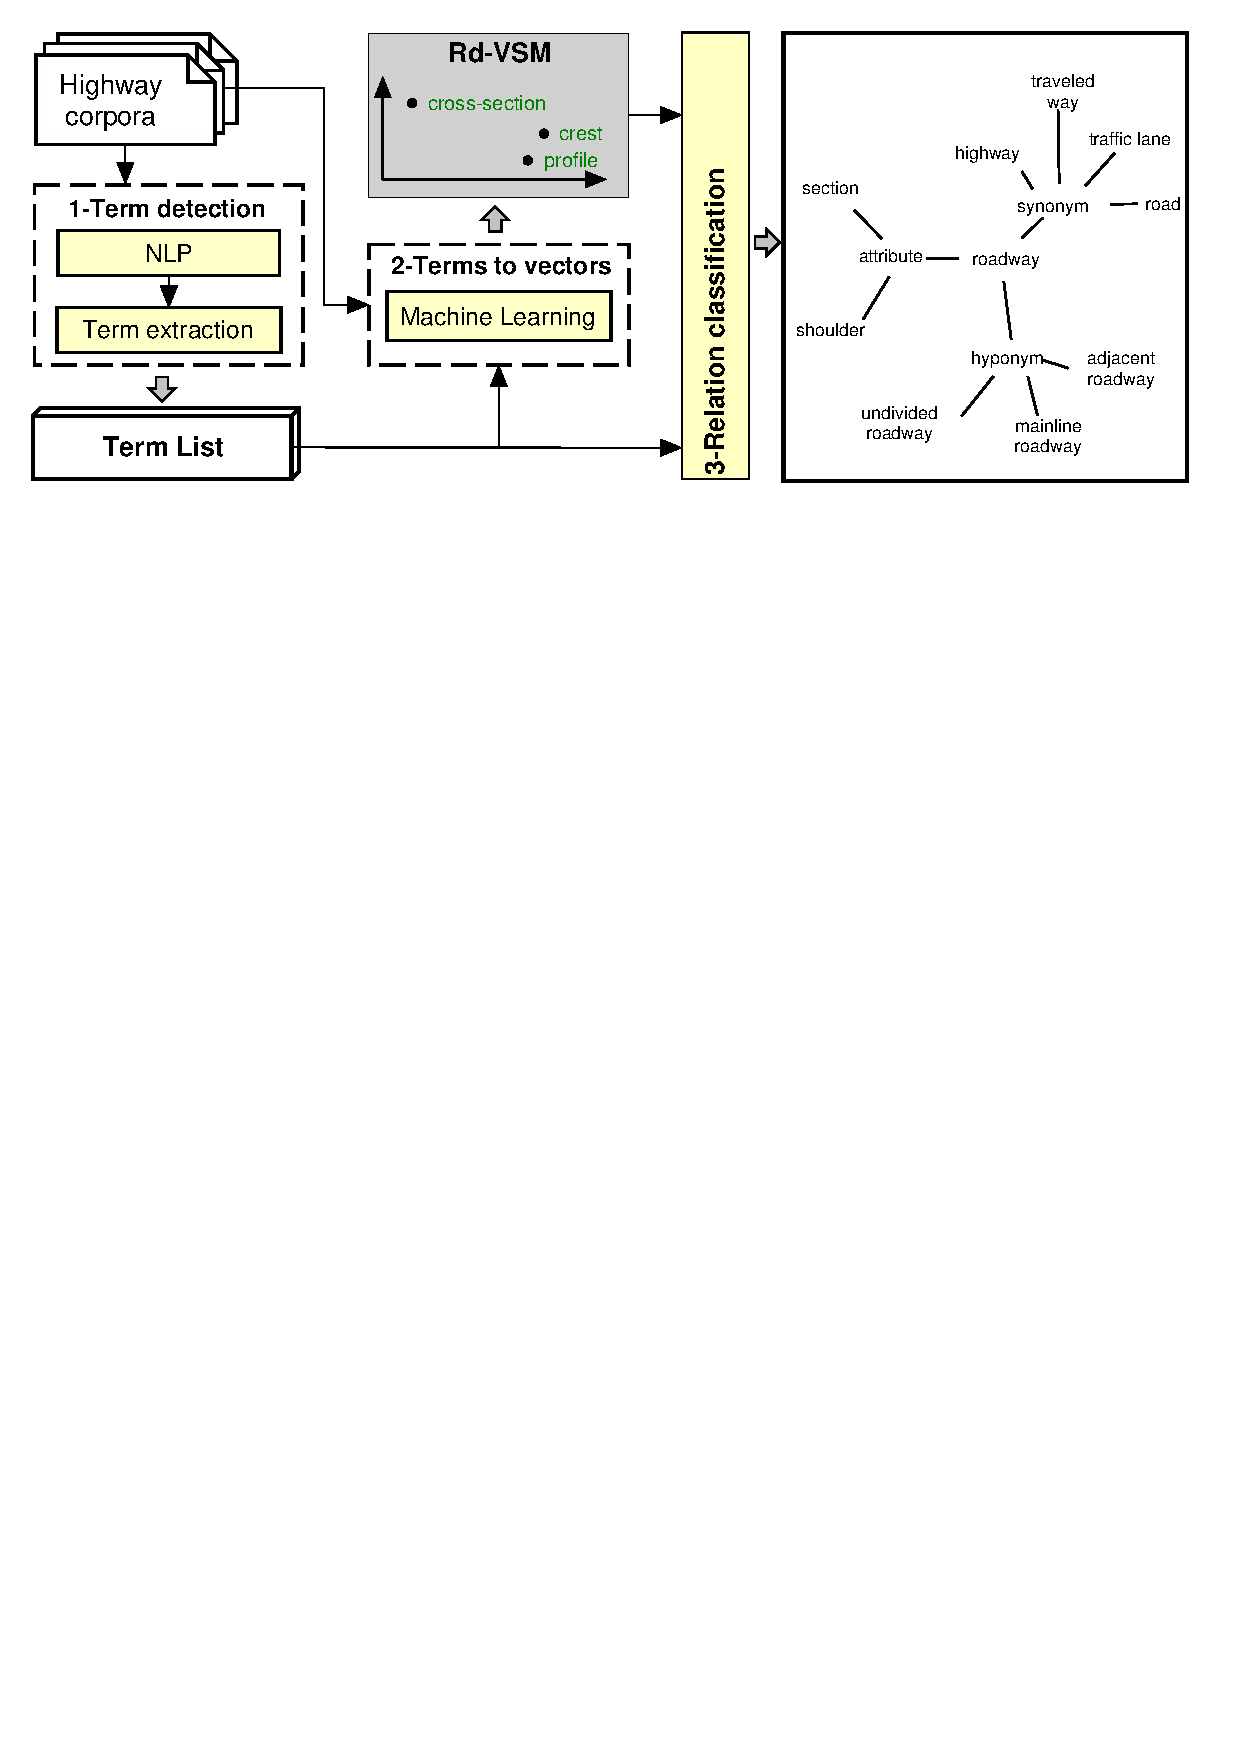
\includegraphics[width=0.95\textwidth]{Figure1_overview_methodology}
	\caption{Overview of the proposed methodology}
	\label{fig:framework}
\end{figure}
%
The ultimate goal of this research is to construct a machine-readable dictionary of American-English technical terms, named InfraLex, for the infrastructure sector. Figure \ref{fig:framework} presents an overview of the methodology proposed to develop InfraLex. The research framework consists of two major modules that are to: (1) train a highway vector space model (H-VSM), and (2) develop an algorithm integrating H-VSM and various linguistic patterns to construct InfraLex. The first module implements several basic NLP techniques (including tokenizing, POS tagging, etc.) and C-value method \cite{frantzi20} to extract highway related technical terms from a highway corpora. The Skip-gram model, an unsupervised machine learning platform proposed by \citeN{mikolov13a}, is then employed to train the semantic similarity between technical terms. The model uses the unlabeled highway corpora as the training dataset. This training process transforms the identified terms into representation vectors in a coordinate space model named H-VSM.  Using this term vector space, the similarity degree between technical terms can be determined; and based on that the list of nearest terms for a given term can be obtained. The second module designs an algorithm for identifying the relation (e.g., synonymy, hypernymy, hyponymy, or attribute) between each item in the nearest list and the target term. The InfraLex lexicon is finally constructed by organizing the domain vocabulary into a network of terms which link to each other through the identified semantic relations. Specifically, the procedure followed to compile the InfraLex dictionary is comprised of the following steps: (a) collect highway technical documents to compose a domain corpus; (b) extract the multi-word terms from the highway corpus; (c) prepare the training dataset for training the H-VSM model; (d) select appropriate values for the training parameters and perform the training of the H-VSM model; and (e) design an algorithm to classify related terms into groups of lexical relations. The below sections discuss these steps in detail.
%\begin{enumerate} [label=(\alph*)]
%\item 
%\item 
%\item 
%\item 
%\item 
%\end{enumerate}
%
%TODO: The preliminary result is presented by. In this paper, the model is extended with larger training datasets and post-processing to reorganize terms in categories which improves the semantic data searching algorithm.
%\section{Highway term space model development} \label{sec:vector-space}
%
%introduction to the distributional vector model, fundamental theory,  the overall process to translate technical terms into vectors representations. the role of vector space allow measure the similarity between 
%TODO: This section presents the extension of the H-VSM developed by the authors' previous work with the extending of training datasets and post-processing of the vector space model.
%
\subsection{Data collection}
%how to collect data, how to clean data to get them readay for training model
%aim text folow remained, flow direction. bottom down, 
%remove heading (chapter, section, subsection), footnote, numerbing, bullets, hyperlink, url, 
As mentioned earlier, H-VSM was trained using a machine learning model which requires a text corpus as the source of the training dataset. The input text corpus was built upon a plethora of highway engineering manuals from the Federal Department of Transportation (DOT) and from 22 State DOTs. These documents in American-English. The technical terms in a guidance document in the engineering field are organized in various formats such as plain text, tables, and equations. Since words in tables and equations are not yet supported by the state-of-the-art NLP techniques, they were removed from the text corpus. The removal of these features would reduce corpus size, but it is necessary since words in tables and equations are not organized in a regular sentence structure and therefore the NLP algorithm may extract unreal noun phrases. The final outcome of this phase is a plain text corpus consisting of 16 million words. This dataset is utilized to extract highway related technical terms which are then trained and converted into representation vectors.
%
\subsection{Multi-word terms extraction}
%
\begin{figure}[t]
	\centering
	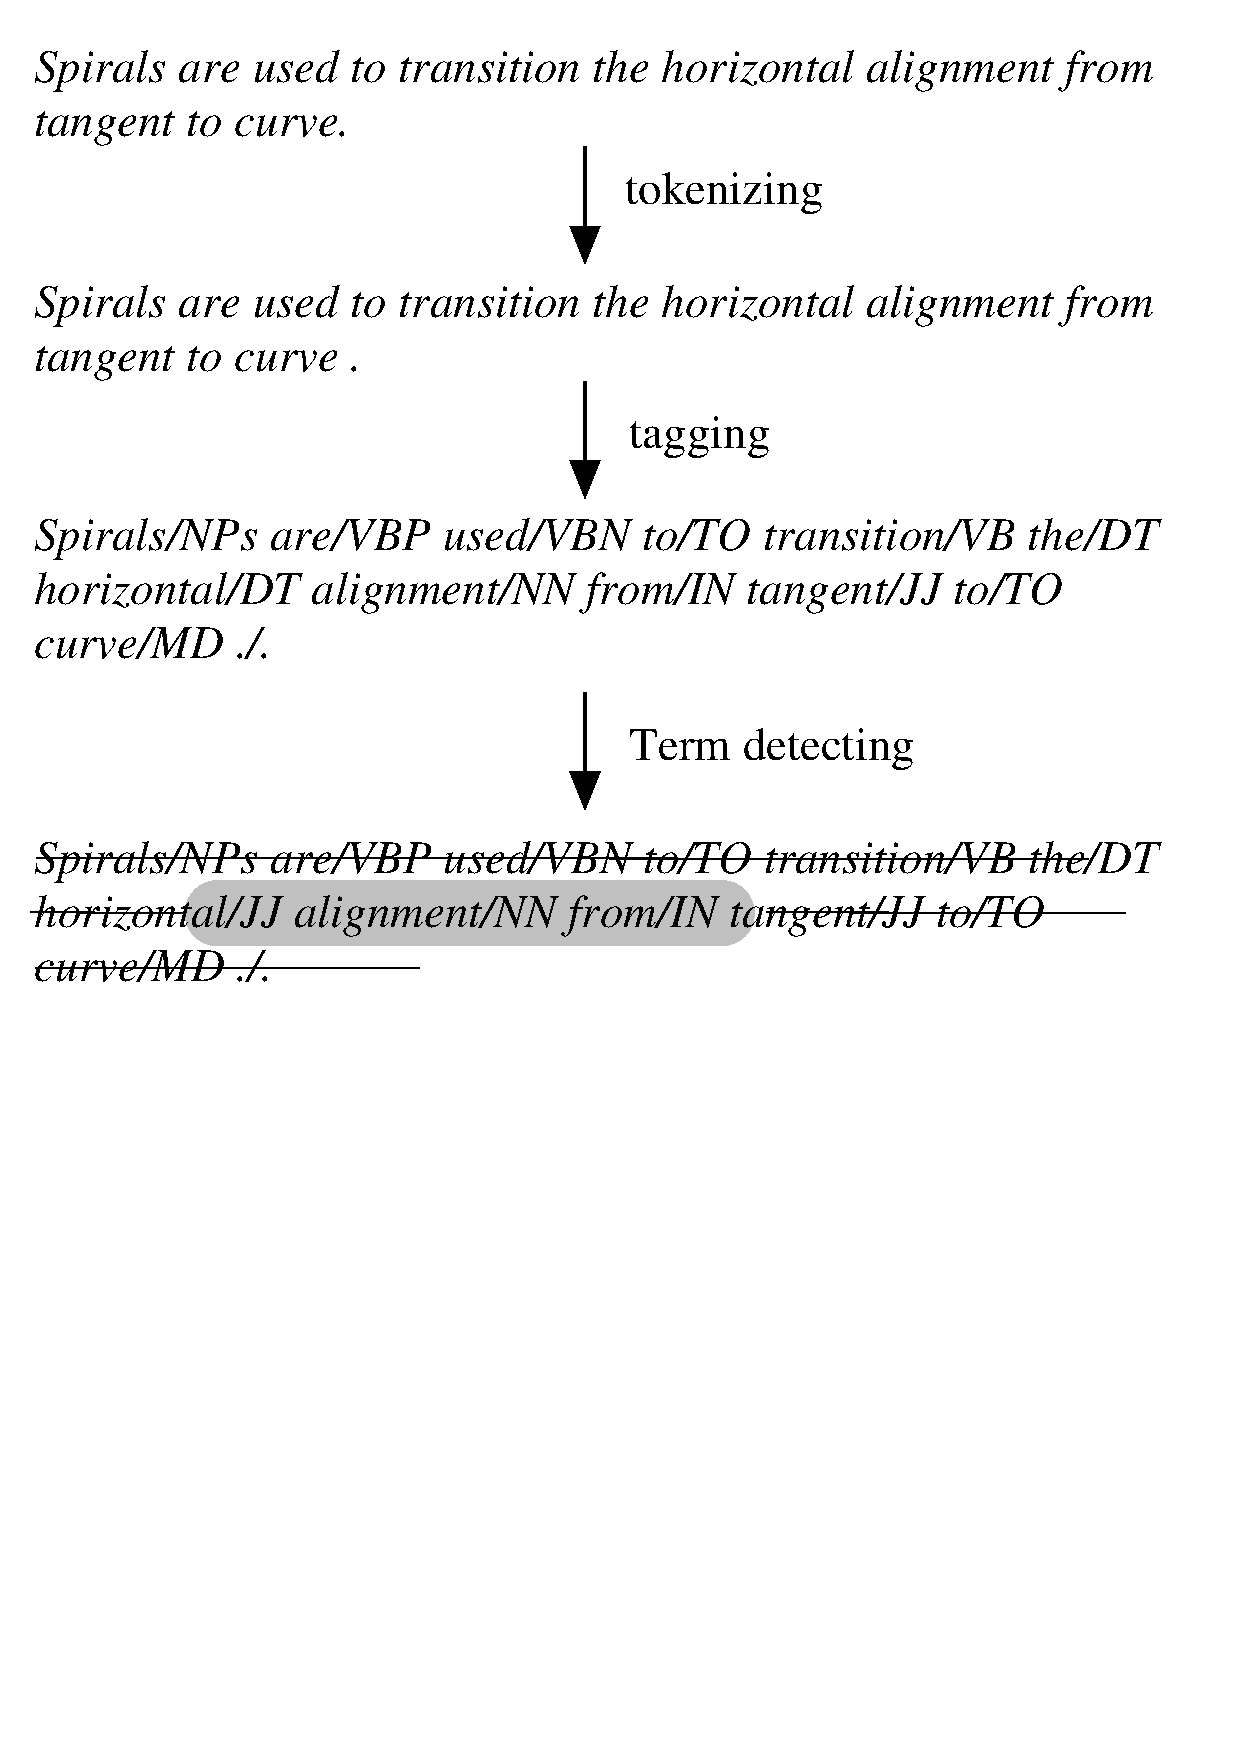
\includegraphics[width=0.45\textwidth]{Figure2_term_extraction}
	\caption{Linguistic processing procedure to detect technical terms}
	\label{fig:np_detect}
\end{figure}
%
A technical term can be a noun (e.g., roadway, lane, etc.) or be a noun phrase composed of multiple words (e.g., right of way, at grade intersection, etc.). The meaning of multi-word terms may not be directly interpreted from the meanings of their single words. In order for the Skip-gram model to learn the semantics of multi-word terms, every occurrence of multi-word terms in the corpus needs to be detected and replaced with connected blocks of word members so that they can be treated as single words. This research utilizes OpenNLP, NLP package, to process the collected corpus and detect sequences of words that match pre-defined noun phrase patterns. Figure \ref{fig:np_detect} presents the process of detecting technical terms from the set of highway technical documents. The process includes the following steps. 
\par
\begin{enumerate} [label=\roman*]
	\item \textbf{Word tokenizing:} In this step, the text corpus is broken down into individual units (also called tokens) using OpenNLP Tokenizer.
	\item \textbf{Part of Speed (POS) tagging:} The purpose of this step is to determine the Part of Speech (POS) tag (e.g., noun, adjective, verb, etc.) for each token of the tokenized corpus obtained from the previous step. A set of POS tags can be found in the Penn Treebank \cite{marcus93}.
	\item \textbf{Noun phrase detection:} Linguists argue that a technical term is either a noun (e.g., road) or a noun phrase (NP) (e.g., right of way) that frequently occurs in domain text documents \cite{justeson95}. Thus, NPs are good multi-word term candidates. Table \ref{table:term_filter} presents the proposed extraction patterns which are modified from the filters suggested by \citeN{justeson95} to extract NPs. The tagged corpus is thoroughly scanned, and sequences matching to the noun phrase patterns is collected. 
	%
	In addition, in order to avoid discrimination among the syntactic variants of the same term, for example `roadway' and `roadways', the collected NPs need to be normalized. The following are two types of syntactic variants and the proposed normalization methods.
	\begin{table} [t]
		\caption{Term candidate filters}
		\label{table:term_filter}
		\centering
		\small
		\renewcommand{\arraystretch}{1.25}
		\begin{tabular}{l l}
			\hline
			\textbf{Pattern} & \textbf{Examples}\\
			\hline
			(Adj|N)*N		& road, roadway shoulder, vertical alignment\\
			(Adj|N)*N Prep (of/in) (Adj|N)*N	&	right of way, type of roadway\\
			%(Adj|N)* 'and/or' (Adj|N)*N & vertical and horizontal alignment\\
			\hline
			\multicolumn{2}{l}{\textit{Note:} |, * respectively denote `and/or', and `zero or more'.  } \\
			\hline
		\end{tabular}
		\normalsize
	\end{table}
	%
	\begin{itemize}
		\item \textbf{Type 1} - Plural forms, for example `roadways' and `roadway'. The Porter stemming algorithm \cite{porter80}, which can allow for automated removal of suffixes, is applied on the extracted noun phrases to normalize plural nouns (NNS) into single nouns (NN). Since the stemming algorithm affects only on the NNS token of a Noun phrase, the issue of over and under stemming can be minimized/eliminated. %todo: update algorithm so that stemming only occur in the the noun phrase extraction phase, not for the entire corpus.
		\item \textbf{Type 2} - Preposition noun phrases, for example `roadway type' and `type of roadway'. In order to normalize this type of variant, the form with preposition is converted into the non-preposition form by removing the preposition and reversing the order of the remaining portions. For instance, `type of roadway' will become `roadway type'.
	\end{itemize}
	%
	Since NPs with low occurrence frequencies that are unlikely to be technical terms should be automatically eliminated. With the frequency threshold of 2, the list consists of 112,024  terms. The list size drops to 8,922 when a threshold of 50 is used. In this research we used a threshold of 50.
	%
	\item \textbf{Multi-word term candidate ranking and selection:} Multi-word term definition varies between authors, and there is a lack of formal and widely accepted rules to define if a NP is a multi-word term \cite{frantzi20}. There are a number of methods proposed for estimating termhood (the degree that a linguistic unit is a domain-technical concept), such as TF-IDF  \cite{sparck72,salton88}, C-Value \cite{frantzi20}, Termex  \cite{sclano07}. These methods are based on the occurrence frequencies of NPs in the corpus. Among these methods, Termex outperformed other methods on the Wikipedia corpus, and C-Value was the best on the GENIA medical corpus \cite{zhang08}. This result indicates that the C-value method is more suitable for term extraction from a domain corpus rather than a generic corpus. For this reason, the C-value has been widely used to extract domain terms in the biomedical field, for instance studies performed by \citeN{ananiadou20}, \citeN{lossio13}, and \citeN{nenadic02}. Since the corpus used in this study was mainly collected from technical domain documents, C-value would be the most suitable for the termhood determination task. The C-value measure, as formulated in Equation \ref{eq:cvalue}, suggests that the longer a NP is, the more likely that is a term; and the more frequently it appears in the domain corpus, the more likely it will be a domain term.
	% 
	\begin{equation}
	C-value(a)=
	\begin{cases}
	log_2|a|.f(a), & \text{if a is not nested} \\
	log_2|a|(f(a)-\frac{1}{P(T_a)}\sum_{b\in T_a} f(b)), & \text{otherwise}
	\end{cases}
	\label{eq:cvalue}
	\end{equation}
	%
	Where:
	\begin{description}
		\item[a] is a candidate noun phrase
		\item[|a|] is the length of noun phrase \textit{a}
		\item[f] is the frequency of \textit{a} in the corpus
		\item[Ta] is the set of extracted noun phrases that contain \textit{a}
		\item[P(Ta)] is the size of Ta set.
	\end{description}
\end{enumerate}
%
\par
The term extraction process above results in a dataset containing the detected terms along with their c-value termhood scores. These term candidates are ranked by C-value, and the ones that have negative C-values are discarded. %todo: add a picture of excerpt of detected term dataset, 3-column table with the following column names: term, frequency, termhood c-value.
\par
To remove candidates that are unlikely to be real terms, a threshold C-value can be used or the entire candidate list should be manually evaluated by industry experts. Manual evaluation would avoid the removal of real terms but have low C-values. To minimize both laborious work and the number of true terms wrongly discarded, the ranked list of candidate were divided into groups of 100 items. A graduate student with civil engineering background was asked to utilize a bottom-up approach to evaluate group by group and stop at which has a precision of 80 percent. Table \ref{table:term_evaluation} illustrates the evaluation results for several excerpts of the extracted term candidates. The precision values, which represent the percentage of real terms in these groups, are presented in Figure \ref{fig:term_precision}. As shown in the figure, precision values are relatively low for groups with c-values less than 70. To balance between human effort and precision of the final term list, this research applied a manual review on the set of XX automatically extracted terms with c-values less than the threshold of 70 at the bottom of the list.
%To calculate the recall value, expert is required to final all true terms from the corpus \cite{frantzi20}. with the large corpus in this research, it is impossible to do this task. 
%
\begin{table} [t]
	\caption{Excerpts of the extracted candidate terms}
	\label{table:term_evaluation}
	\centering
	\small
	\renewcommand{\arraystretch}{1.25}
	\begin{tabular}{l l l}
		\hline
		\textbf{Term} & \textbf{Termhood} & \textbf{real term?}\\
		\hline
		sight distance		& 9435.314 & yes\\
		design speed & 9052.556 & yes \\
		additional information & 1829.0 & no\\
		typical section & 1801.0  & yes\\
		basis of payment & 1762.478 & no\\
		\hline
	\end{tabular}
	
	\normalsize
\end{table}

\begin{figure}[t]
	\centering
	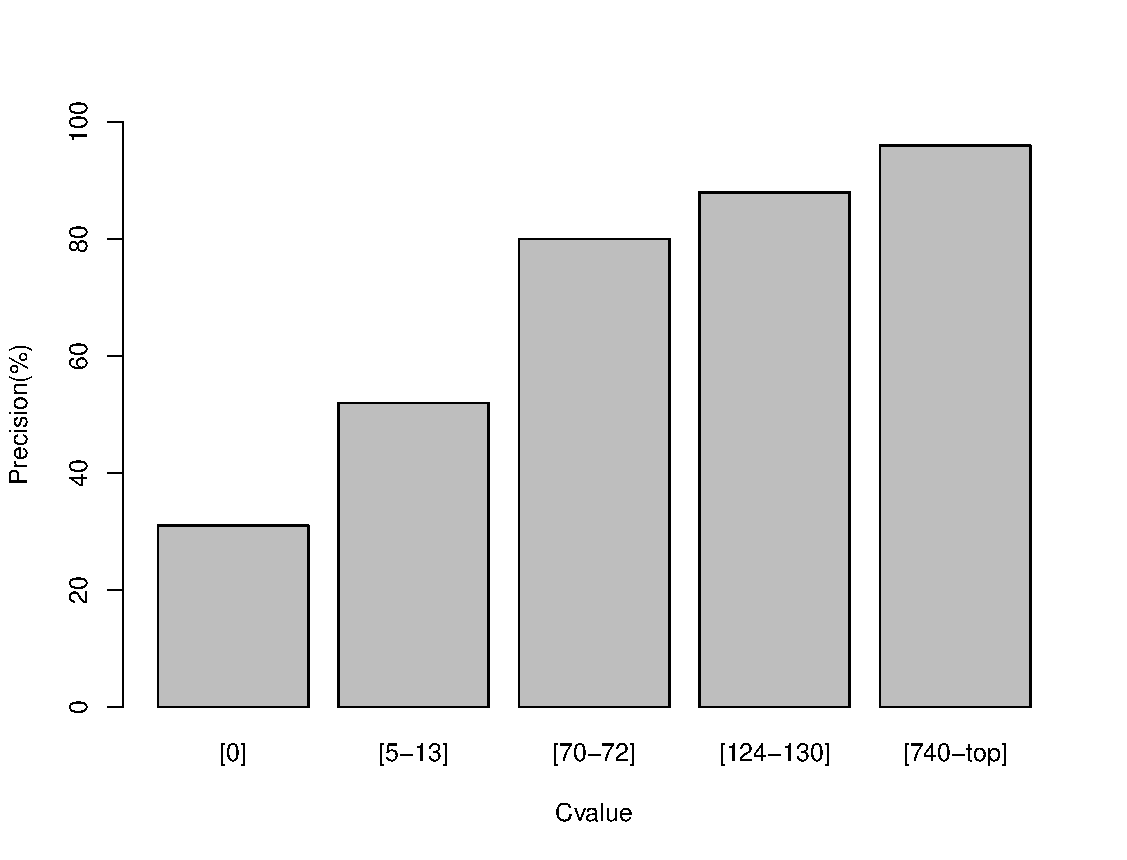
\includegraphics[width=0.5\textwidth]{Figure3_term_precision}
	\caption{Multi-word term extraction evaluation}
	\label{fig:term_precision}
\end{figure}
%
\subsection{Construction of term space model}
%
This step aims at processing the collected text corpus and collecting the training data for developing the H-VSM model. Skip-gram \cite{mikolov13a}, which is an un-supervised machine model, was employed to learn the semantic similarity among words in the text corpus. The Skip-Gram model requires a set of training data in which the input data is a linguistic unit (word or term), and the output data is a set of context words which are closed to the input unit in the corpus. In order to collect this training dataset, the unannotated highway corpus is scanned to capture instances of terms and their corresponding context words. Each occurrence of a word will correspondingly generate a data point in the training dataset.
\par
Before collecting the training dataset, an additional step is needed to handle the issue related to multi-word terms. Since document scanning is on a word-by-word basis, the corpus must be adjusted so that multi-word terms can be treated like single words. To fulfill that requirement, every occurrence of a certain multi-word term in the corpus is replaced with a single unit that is compiled by connecting all the individual words. For instance, `vertical alignment' becomes `vertical-alignment'.
\par
The number of context words to be collected is dependent on the window size that limits how many words to the left and the right of the target word. In the example sentence below, the context of term `roadway' with the window size of 5 will be the following word set \{bike, lane, width, on, a, width, no, curb, gutter\}. Any context word that is in the stop list (the list contains frequent words in English such as `a', `an', and `the' that have little meaning) will be neglected from the context set.
%
\begin{center}
	"The minimum [bike lane width on a \underline{roadway} with no curb and gutter] is 4 feet."
\end{center}
%
%todo: word2vec, brief introduction about word2vec
%skip-gram model
%how to modify the method of selecting conext words
%java program
%
\begin{figure}[t]
	\centering
	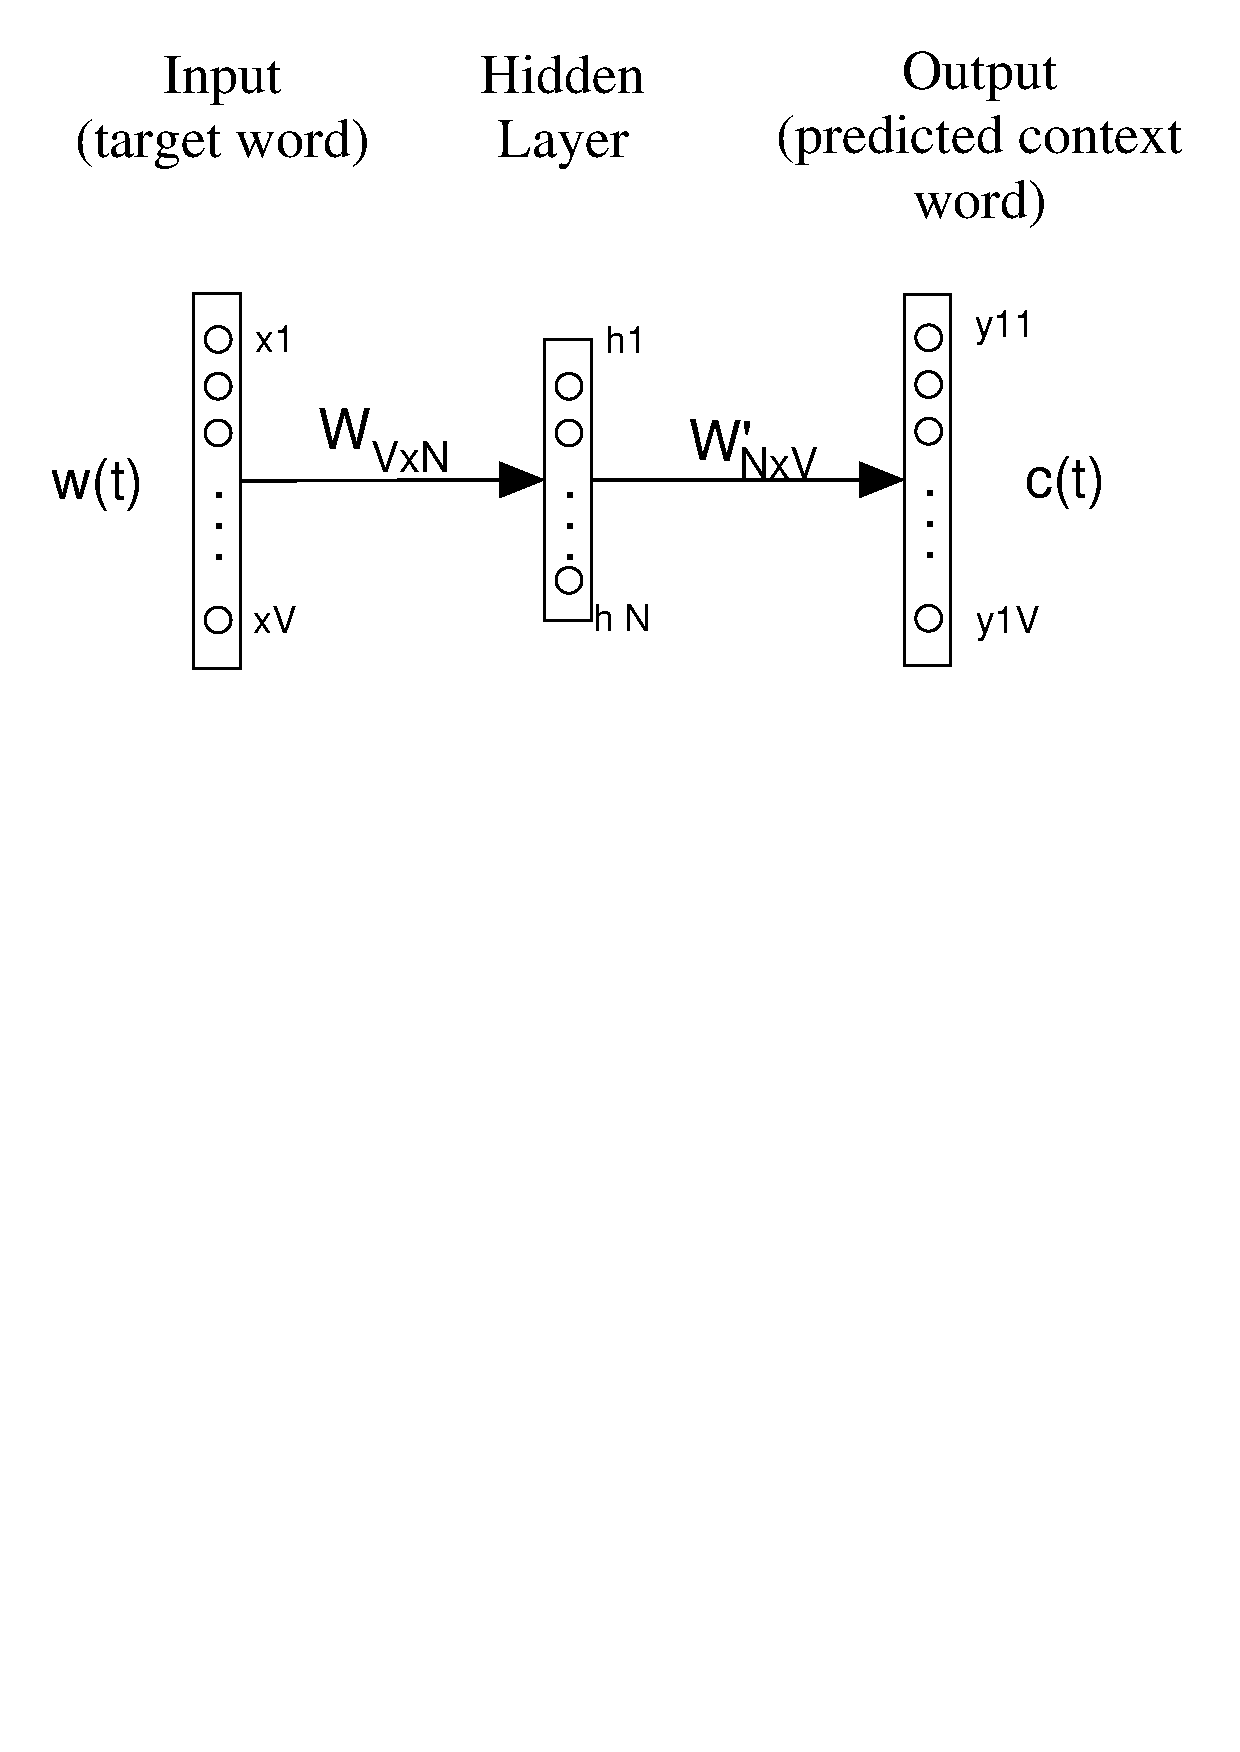
\includegraphics[width=0.45\textwidth]{Figure4_skip-gram-model}
	\caption{Skip-gram model}
	\label{fig:skip-gram}
\end{figure}
%
The semantic similarity is trained using the Word2vec module in the Apache Spark MLlib package \cite{apache16}, an emerging open-source engine, which is based on the Skip-gram neural network model \cite{mikolov13a}. Figure \ref{fig:skip-gram} shows the learning network when the context set includes only one word, where \textit{V} and \textit{N} respectively denote the corpus vocabulary and hidden layer size. In this model, a word in the corpus vocabulary is encoded as a 'one-hot' vector which is a vector in which only one elements at the index of the word in the vocabulary is set one, and all other items are zero. For example, the one-hot vector of $k^{th}$ word in the vocabulary with the size of V will be {x1=0, x2=0, ...,xk=1,...xV=0}. The outcome of this machine learning process is a set of term representation vectors  in an N-dimension coordinate system. as we can see, the similarity among predicted context vectors are decided by the similarity of the corresponding \textit{representation vectors}. each row of the W matrix which is the output of the learning process, is a representation vector of a word in the corpus vocabulary. The similarity among these vectors represent the similarity of the context of the corresponding words. 
%
\begin{enumerate}
	\item $k^{th}$ input word : $[x_k]_{1.V} = [x_1=0, x_2=0,...,x_k=1,..., x_V=0]$ which is an one-hot vector.
	\item Hidden vector:$[h]_{1.N} = [x_k]_{1.V}.W_{V.N} = [w_{k1},w_{k2},..., w_{kN}]= v_{wk}$ which is equivalent to the $k^{th}$ row of the W matrix since the input vector is a 'one-hot' vector. The $v_{wk}$ vector is called the input \textit{representation vector} of the input word $k^{th}$.
	\item Predicted context vector: $[y_k]_{1.V} = v_{wk}.W'_{N.V}$. 
\end{enumerate}
%
\par
The model includes three major parameters that are \textit{frequency threshold}, \textit{hidden layer size} and \textit{window size} (see Table \ref{table:nn-parameters}). To eliminate those data points with low frequencies of occurrence that are unlikely to be technical terms, Word2vec allows for the use of \textit{frequency threshold}. Any word with the rate lower than the limit will be ignored. \citeN{rehurek14} suggests a range of (0-100) depending on the data set size. Setting this parameter high will enhance the accuracy, but many true technical terms would be out of vocabulary. A preliminary study based on the preliminary corpus with only several millions of words shows that with the frequency of 20, there are very few non-technical terms involved in the training dataset. Hence, with the larger dataset to be collected, this parameter can be higher and up to around 50. The second important parameter is \textit{layer size} which determines the number of nodes in the hidden layer. This parameter highly affects the training accuracy and processing time. A larger layer size is better in terms of accuracy, but this will be paid off by the running time. The reasonable values for this parameter are from ten to hundreds \cite{rehurek14}. The final major parameter, \textit{context window size}, decides how many context words to be considered. Google recommends the size of 10 for the Skip-gram model \cite{google2016}. These parameters are subject to be changed so that the best model can be achieved. The effects of these parameters on the model performance are discussed in Section \ref{sec:eval_infralex}.
%
\begin{table} [t]
	\caption{Skip-gram model parameters}
	\label{table:nn-parameters}
	\centering
	\small
	\renewcommand{\arraystretch}{1.25}
	\begin{tabular}{l l}
		\hline
		\textbf{Parameter} & \textbf{Value}\\
		\hline
		Frequency threshold & 50-100\\
		Hidden layer size		&	100-500\\
		Context window size	&	5,10,15\\
		\hline
	\end{tabular}
	\normalsize
\end{table}
%
\par
Figure \ref{fig:hvsm} presents the term space model of H-VSM derived from the training process when the parameters are set 50, 300 and 10 respectively. H-VSM currently consists of more than 6,000 technical terms. In this model, each technical term is represented as a vector in a high dimensional space. Since the term representation vectors are in a multi-dimensional space; to present the space in 2D graph, PCA (Principle Component Analysis) was used to reduce the size to 2.
\par
The similarity between terms in the H-VSM model can be measured by the angle between two word representation vectors (Equation \ref{equ:cosin_sim}) or the distance between two word points (Equation \ref{equ:dis_sim}). Figure 5 illustrates the clustering of terms by their distances. In this figure, an \textit{inlet} can be inferred to be more similar to an \textit{outlet} (blue) than a \textit{sidewalk} (green). Using this technique, the most similar terms for a given term can be obtained. Table \ref{table:nearest_example} shows a partial ranked list of the nearest terms of `roadway' in order of similarity score.
%
\begin{figure}[t]
	\centering
	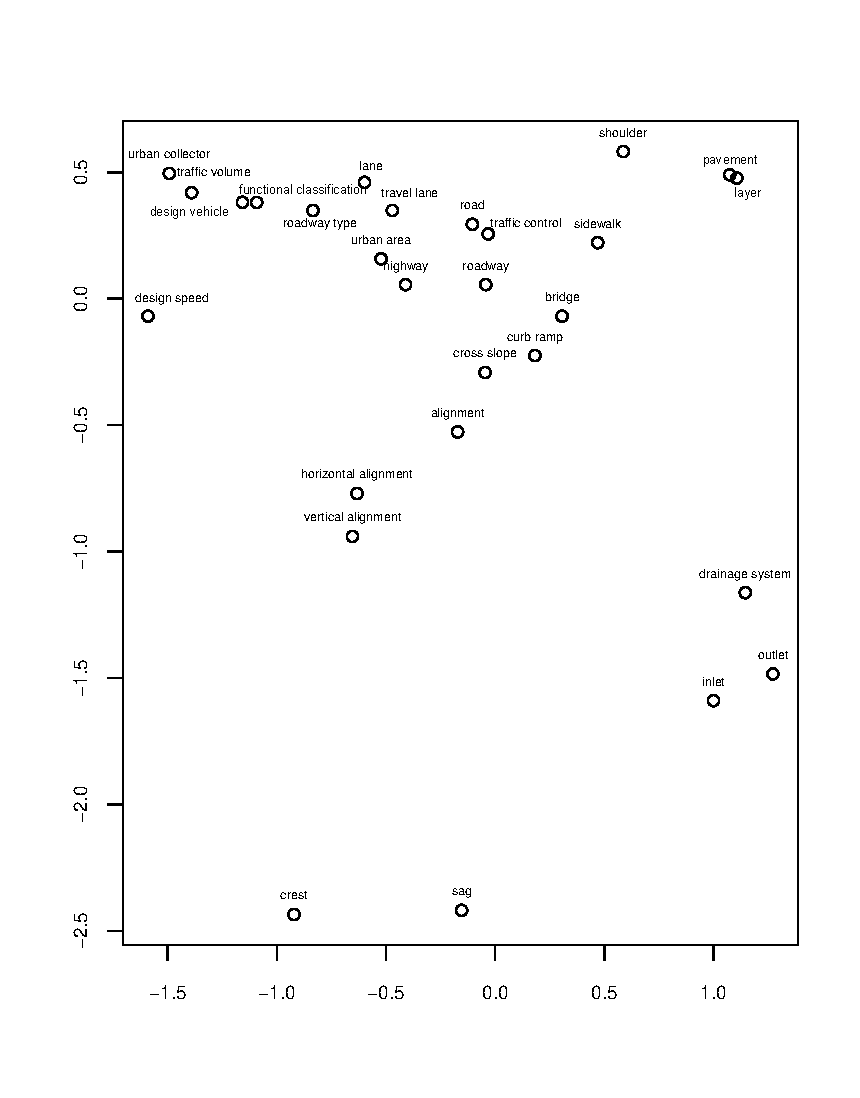
\includegraphics[width=0.95\textwidth]{Figure5_hvsm_space}
	\caption{Highway term space model (H-VSM)}
	\label{fig:hvsm}
\end{figure}
%
\begin{equation}
\label{equ:cosin_sim}
cosine\_similarity = \frac{A.B}{||A||.||B||}
\end{equation}
%
\begin{equation}
\label{equ:dis_sim}
dis\_similarity =\sqrt{(xA_1-xB_1)^2+(xA_2-xB_2)^2+...+(xA_n-xB_n)^2}
\end{equation}

Where: n is the hidden layer size.
%
\begin{table} [t]
	\caption{Examples of top nearest terms}
	\label{table:nearest_example}
	\centering
	\small
	\renewcommand{\arraystretch}{1.25}
	\begin{tabular}{l l l  l}
		\hline
		\textbf{Term} & \textbf{Nearests} & \textbf{Cosine} &\textbf{Rank}\\
		\hline
		roadway			& highway & 0.588 & 1\\
		& traveled-way & 0.583 & 2\\
		& roadway-section & 0.577 & 3\\
		& road & 0.533 & 4\\
		& traffic-lane & 0.524 &5\\
		& separating & 0.522 &6\\
		& adjacent-roadway & 0.519 & 7\\
		& travel-way & 0.517 & 8\\
		& entire-roadway & 0.513 & 9\\
		& ...&...& ...\\
		& roadway-shoulder & 0.505 & 12\\
		& roadway-cross-section & 0.491 & 18\\
		& undivided & 0.452 & 37\\
		& mainline-roadway & 0.450 & 42\\
		\hline
	\end{tabular}
	\normalsize
\end{table}

\subsection{Construction of term lexical hierarchy}
The purpose of this module is to construct Infralex, a lexicon of civil engineering technical terms. A lexicon, also known as a lightweight knowledge base, typically includes terms and relations. The core relations of a lexicon are synonym (meaning equivalence), hypernym-hyponym (also known as IS-A or parent-child relation), attribute (concept property), and association (e.g. part-of) \cite{jiang1997semantic,lee13}. Two terms that relate each other through these semantic relations would have a high similarity score. Therefore, the top nearest terms resulted from H-VSM would be a great starting point for detecting relations between technical terms. Table \ref{table:nearest_example} illustrates a list of nearest terms of `roadway'. In this list, the true synonyms are `highway' (1), `traveled-way' (2) and `road' (4); the attributes include `roadway-section' (3), `roadway-shoulder' (12); and `adjacent-roadway' (7) and `undivided' (37) are hyponyms which show different types of roadway.
\par
The specific objective of this task is to detect the semantic relations among terms which are used for rearranging the nearest terms obtained from the H-VSM model. Algorithm \ref{alg:term_class} shows the design pseudo code for classifying the nearest terms of a given target term. The algorithm utilizes linguistic rules and clustering analysis to organize the nearest list into the following three groups: (1) attribute, (2) hyponym, and (3) synonym/sibling. The algorithm, first detects terms belonging to the first two categories using linguistic patterns. The filter rules to detect these relations are presented in Table \ref{table:attribute_pattern}. For a multi-word term matching pattern 1, we can infer that \textit{Noun1} is an attribute of concept \textit{Noun2}; and \textit{Noun2} is an attribute of \textit{Noun1} in the pattern 2. Pattern 3 is for detecting hyponyms where the matched NP is a hyponym of \textit{Noun2} concept.  The remained nearest words will fall into the third group. However, some of them have far or even no relation with the target word. In order to address this issue, this research employed the K-mean clustering algorithm \cite{macqueen67} to split the remained list into three distinct layers based on the similarity score. The terms in the last group are unlikely to be a synonym or sibling; and thus, are removed from the nearest list. The output of the proposed algorithm is a list of classified nearest terms. Table \ref{table:term_clustering} shows one example for the output retrieved from the algorithm. 
%In contrast, since synonym recognition is well known as the process of evaluating the sharing of common attributes, hypernyms, and hyponyms, this process will rely on the results from the detection of other relations. This task will first detect the following relations (hypernyms, hyponyms and attributes) and then use them as features to find synonyms.
%
\begin{algorithm}[h]
	
	\caption{Near term classification algorithm}\label{alg:term_class}
	\begin{algorithmic}[1]
		\State \textbf{Inputs}: term \textit{t}, list of nearest terms \textit{N}, full list of terms \textit{F}
		\State \textbf{Output:}: Classified list of terms \textit{C}
		\Procedure{Term classification procedure}{}
		%\State $\textit{n} \gets \text{size of }\textit{W}$
		%\State $\textit{m} \gets \text{size of }\textit{T}$
		\State $\textit{Att} \gets \text{list of attributes}$
		\State $\textit{Hyp} \gets \text{list of hyponyms}$
		\State $\textit{Syn} \gets \text{list of synonyms}$
		\State $\textit{w} \gets \textit{null}$
		\ForAll {$n \in N$}
		\If {$n$ contains \textit{t}}
		\State $w \gets n$
		
		\Else
		\ForAll {$f \in F$}
		\If {$f$ contains both $n$ and \textit{t}}
		\State $w \gets f$	
		\State Break for
		
		\EndIf
		\EndFor
		\EndIf
		
		\If {$w$ matches \textit{Attribute pattern}}
		\State add $w$ to \textit{Att}
		\ElsIf {$w$ matches \textit{Hyponym pattern}}
		\State add $w$ to \textit{Hyp}
		\Else
		\State add $w$ to \textit{Syn}
		\EndIf
		\EndFor
		\State Cluster \textit{Syn} and discard low relevant terms
		
		\EndProcedure
	\end{algorithmic}
\end{algorithm}
%
%\subsection{Attribute and hyponym patterns}
%
\begin{table} [t]
	\caption{Patterns to extract attributes and hyponyms}
	\label{table:attribute_pattern}
	\centering
	\small
	\renewcommand{\arraystretch}{1.25}
	\begin{tabular}{l l l}
		\hline
		\textbf{Relation} & \textbf{Pattern} & \textbf{Example}\\
		\hline
		Attribute &	Noun1 of Noun2 & the width of the road\\
		& Noun1 Noun2	&	road width, project cost\\
		Hypernym-hyponym & Noun1 Noun2 & vertical alignment isA alignment\\
		\hline
	\end{tabular}
	\normalsize
\end{table}
%
%After the candidate list is refined, the frequency of occurrence for each candidate will then be used to compute the degree that term 'a' is an attribute of concept 'c'. If 'a' is a typical attribute of 'c', it should frequently occur in the corpus. Each concept 'c' will correspondingly have a list of attribute candidates (called list A) and their frequency of occurrences. The likelihood that 'a' is an attribute of concept 'c' is estimated using the normalized probability formula (see Equation \ref{eq:attribute}). The attribute candidates for each concept will be ranked by the likelihood measure and the top list over a threshold value will be accepted as typical attributes. 
%\begin{equation}
%P(a|c)=\frac{n(c,a)}{\sum_{a* \in A} n(c,a)}
%\label{eq:attribute}
%\end{equation}
%\subsection{Synonym/sibling and functional relation recognition}

%
\begin{table} [t]
	\caption{An example in InfraLex}
	\label{table:term_clustering}
	\centering
	\small
	\renewcommand{\arraystretch}{1.25}
	\begin{tabular}{l l l l l}
		\hline
		\textbf{Term}	&\textbf{Relation Group}	& \textbf{Nearests} & \textbf{Cosine} & \textbf{Rank}\\
		roadway			&Synonym					& highway & 0.588 & 1\\
		&							& traveled-way & 0.583 & 2\\
		&							& road & 0.533 & 4\\						
		&							& traffic-lane & 0.524 &5\\ 						
		&							& travel-way & 0.517 & 8\\  \cmidrule{2-5}
		&Attribute					& separating & 0.522 &6\\
		&							& roadway-section & 0.577 & 3\\						
		&							& roadway-shoulder & 0.505 & 12\\
		&							& roadway-cross-section & 0.491 & 18\\\cmidrule{2-5}						
		&Hyponym					& adjacent-roadway & 0.519 & 7\\
		&							& entire-roadway & 0.513 & 9\\
		&							& undivided & 0.452 & 37\\
		&							& mainline-roadway & 0.450 & 42\\
		\hline
	\end{tabular}
	\normalsize
\end{table}


\section{Performance evaluation} \label{sec:eval_infralex}
%evaluation method
This section presents a performance evaluation of InfraLex on the ability to identify synonyms. In this experiment, a gold standard  is used. The gold standard consists of 70 sets of synonyms (both single and multi-word terms) which were examined and extracted from a Wikipedia transportation glossary \cite{wikipedia16}. The developed Infralex model was employed to find the synonym for a given input term. The automatically identified synonym is the nearest word in the synonym/sibling lexical group. The evaluation outcome returns ``true'' if the automatically identified synonym belongs to the actual synonym set of the tested term in the golden standard. The performance was evaluated using the following three measures including precision, recall, and f-measure. Precision refers the accuracy in the conclusions made by the system, and recall reflects the coverage of domain terms of the system. The F score, which is a combined measure of precision and recall, presents the overall performance of a system. 
%
\begin{align} 
&Precision = \frac{\text{number of correctly detected synonyms}}{\text{total detected terms}}  \\
&Recall = \frac{\text{number of correctly detected synonyms}}{\text{total terms}}  \\ 
&F-measure = \frac{2.Precision.Recall}{Precision+Recall}
\end{align}
%results
\begin{table} [b] 
	\caption{Effects of training parameters on performance of synonym matching}
	\label{table:eval_syn_par_effect}
	\centering
	\small
	\renewcommand{\arraystretch}{1.25}
	\begin{tabular}{l l l l l }
		\hline
		\hline
		\textbf{Parameter} & \textbf{Model} & \textbf{Precision (\%)}  & \textbf{Recall(\%)} & \textbf{F (\%)}\\
		\hline
		Baseline	&	50-100-5	&79		&53		&63\\
		\hline
		\textbf{Window size}	&\textbf{50-100-\underline{10}}	&\textbf{81}		&\textbf{54}		&\textbf{65}\\
		&50-100-\underline{15}	&81		&54		&65\\
		\hline		
		Frequency threshold	&\underline{75}-100-5	&74		&50		&60\\
		&\underline{100}-100-5	&77		&51		&62\\
		\hline
		Hidden layer size	&50-\underline{200}-5	&79		&53		&63\\
		\hline
		\hline
	\end{tabular}
	\normalsize
\end{table}
%
%synonym matching peformance result
Table \ref{table:eval_syn_par_effect} shows the performance with various training model settings. The parameters of the baseline model are 50, 100 and 5 respectively for frequency threshold, hidden layer and window size. The authors changed these parameters one by one and kept the other ones unchanged to evaluate their effects to the model performance. As presented in the table, the increase of window size to 10 or 15 resulted in the best model which has a precision of 81\% and an F-measure of 65\%. The change of other parameters did not improve the performance. Especially, the increase of frequency threshold value has negative impact. 
%compared to the previous publication by the authors, this algorithm has been improved with significantly higher accuracy. the post-processing is one reason for the out-performance of the proposed method.  
%
%result
\begin{table} [b] 
	\caption{Comparison of synonym matching performance between Wordnet and InfraLex}
	\label{table:eval_syn_vs_Wordnet}
	\centering
	\small
	\renewcommand{\arraystretch}{1.25}
	\begin{tabular}{l l l l }
		\hline
		\hline
		\textbf{Lexicon} & \textbf{Precision (\%)}  & \textbf{Recall(\%)} & \textbf{F (\%)}\\
		\hline
		Wordnet	&76 	&40 	&52\\	
		\textbf{InfraLex} &\textbf{81}	&\textbf{54}		&\textbf{65}\\	
		\hline
		\hline
	\end{tabular}
	\normalsize
\end{table}
\par
The proposed model was also compared with the generic Wordnet database. Table \ref{table:eval_syn_vs_Wordnet} presents the comparison of performance between InfraLex (with the 50-100-10 setting) and Wordnet. As shown, InfraLex outperforms Wordnet in all measures, and the combined F-measure is significantly improved (65\% compared to 52\%). The biggest contribution to the improvement of the overall F-measure is the recall value which represents a better coverage of domain vocabulary of InfraLex. 
%attribute  hyponyms and attributes. finding performance
%for attribute and hyponym only precision is determined. to determine the recall require of all possible true attributes for a concept which is challenging and unrealistic task, this research evaluate the accuracy of the extracted attributes. this largely depend on the size and the variety of discipiline covered in the corpus. select of one in each set of synonyms in the gold standard and  humam evaluate attribute and non-attribute. the performance in measure using Equation which represent the percentage of correctly extracted attribute/hyponym. 

%
\section{Discussions} \label{sec:dis}
%contribution of the research
the proposed method to construct lexicon for the construction industry enable a quick translation of text documents to lexicon. The application of the method for roadway domain, a large dataset of terminology with more than 6000 terms have been quickly capture and the relations between terms are be able extracted as well. the research is expected to leverage the and scale up the whole infrastructure level to developed a comprehensive machine readable dictionary for the industry which data integrating and sharing systems can eliminate any terminology mismatches when integrating data from multiple sources. 
%potential application
%todo: refer two research related to NLP in which the first step is to develop lexicon, or other semantic similarity algorithm.
The lexicon dataset developed in this study is expected to become a fundamental resource for a variety of NLP related studies in the civil infrastructure domains. InfraLex can serve as a machine-readable dictionary of domain technical terms. NLP based platforms can utilize this resource for term sense analysis which is crucial for text mining to extract meaningful information from text documents, information retrieval, or natural language based human-machine interaction. Some specific examples of these potential applications are as follows. First, information retrieval systems can use the semantic relations provided by InfraLex to classify project documents by relevant topics by analyzing the keywords in the documents. Second, questionnaire designers can utilize InfraLex to search for synonyms so that appropriate terms can be selected for specific groups of potential respondents who might be from multiple disciplines or regions. Another application is that the query systems for extracting data from 3D engineered models would be able to find alternative ways to query data when users' keywords do not match any entity in the database. Since users have different ways and keywords to query data, the ability to recognize synonyms and related concepts of a query system would provide flexibility to the end user. Also, the developed InfraLex lexicon would enable the matching data items such as (e.g., cost, productivity, etc.) when integrating data from distinct departments or states to develop a national database. This study is also expected to fundamentally transform the way human interacts with machine as technical terms which are a basic unit of human language can be precisely understood by computer systems. Instead of using computer languages, the end user can use natural language to communicate with computer systems.
%add discussions
In order to enable computer to understand human language, a machine-readable dictionary which defines meanings of relevant vocabulary is required. therefore, the developed lexicon can be used by NLP applications for the domain of infrastructure. 
\par
%
%limitation and potential direction for improvement
The current study has some limitations that may contribute the low overall performance. First, the highway corpus is still relatively small with only 16 million words, compared to the corpus sizes in other domains with billions of words. Since the recall value largely depends on the corpus size, the expansion of the highway corpus would enable more technical terms to be covered in InfraLex. Future research is needed to enhance the performance of InfraLex by enlarging the data training set in both size and the number of disciplines involved throughout the life cycle of a highway project, such as asset management, project programming, construction management. The corpus also needs to cover other types of transportation assets like bridge, tunnel, railway, culvert, etc. Another work that can potentially improve the model performance is to distinguish synonym and sibling which are still in the same group in the InfraLex system. When these two lexical relations are separated, the possibility of recognizing a wrong synonym will be reduced; and consequently, the precision value would be enhanced.
%add limitation
%todo: discussion on what is a good precision and f-measure
%todo: the issue of tow polysymy has not been addressed. synonymy has been addressed. 
\section{Conclusions} \label{sec:conclns3} 
Data manipulation from multiple sources is a challenging task in infrastructure management due to the inconsistency of data format and terminology. The contribution of this study is a digital lexicon of highway related technical terms (named InfraLex) which can enable a computer to understand semantic meanings of terms.  This research employs advanced NLP techniques to extract technical terms from a highway text corpus which is composed of 16 million words built on a collection of design manuals from 22 State DOTs across the U.S. Machine learning was used to train the semantic similarity between technical terms. An algorithm was designed to classify the nearest terms resulted from the semantic similarity model into distinct groups according to their lexical relationships. This algorithm was employed to develop the InfraLex database. 
\par
The developed lexicon has been evaluated by comparing the results obtained from the computational model and a man-crafted gold standard. The result shows an accuracy of over 80 percent.  The best model is associated with the training parameters of 50, 100 and 10 respectively for frequency threshold, hidden layer size, and window size. Although significant improvement is shown in comparison with the existing thesaurus databases, the overall performance is not relatively high. This might be due to the size of the training data. Future research will be conducted to expand the highway corpus to further disciplines such as asset management, and transportation operation. 
\par
The research opens a new gate for computational tools regarding natural language processing in the highway sector. InfraLex would enable computer systems to understand terms and consequently transform the way human interacts with computer by allowing users to use natural language. 

\bibliography{mybib}
%
%
\end{document}

